The high priority requirements of this project have been met, with the possible exception of using a commonly found file format to output the summaries. There are several pieces of evidence and justification for this. One of the requirements was to reduces the quantity of data through summarising it, while maintaining useful information. The information in the final summaries produced has been chosen based on research into past studies completed using the CRAWDAD datasets. Key data which was used in the studies such as the encounters between devices, device identifications for the endpoints, and encounter duration are all present in the summary output. It can also be shown quantitatively that the quantity of data has been significantly reduced from the input data to the summarisation, figure \ref{fig:size_red} shows how the quantity of data is reduced for each building in the dartmouth/campus data. On average this is a reduction in the number of bytes of over 99\%. 

\begin{figure}[h]
    \centering
    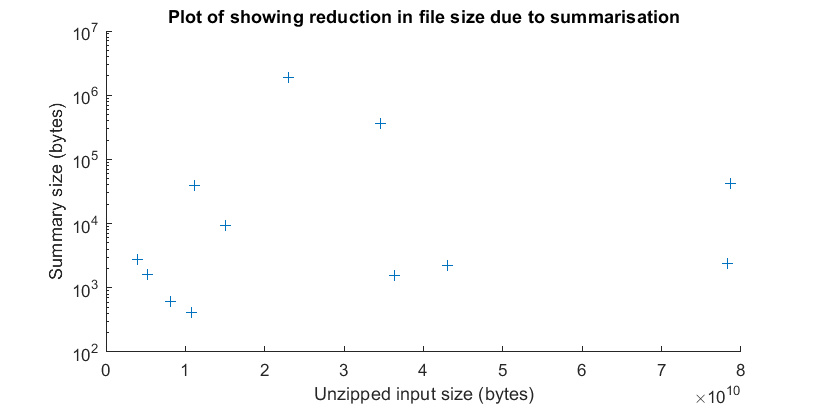
\includegraphics[width=\textwidth]{size_red.png}
    \caption{This figure shows the number of bytes in the unzipped input files compared to the bytes in the output file. This data was collected over the dartmouth/campus dataset where each input is the network trace of a specific campus building over a single measurement period. It can be seen that the number of bytes per files is reduced by between 3 and 8 orders of magnitude. This is a minimum reduction of 99.992\%.}
    \label{fig:size_red}
\end{figure}

This reduction in size also contributes somewhat to meeting the second requirement specified; the summary should be able to be processed more efficiently than the original data. Such a reduction in size denotes a reduction in the complexity and information content of the data. Assuming that the information required for further processing is still present in the summary, it will be much quicker to find in future processing tasks. In addition to this the output of the tool is a simple CSV format, meaning that many tools and software packages will be compatible with it.
The final high priority requirement was that the output should use a common format which is appropriate to the context of this project. The use of specific data fields in the output are justified fully in section 3.2, the fields were chosen with consideration to past use of the dartmouth/campus datasets with the aim to include only information which was seen to be frequently relevant during previous research using the datasets. Although a CSV file could be argued to be a common format, it has little to no specific relevancy to the field of mobility research, requiring that specifically developed tools would need to be developed to further process the summaries produced by this project. 

Summaries are able to be produced based on both syslog or tcpdump/pcap input files. The output produced using each input type is of the same format, however the format of the input needs to be specified at run time using an argument. This meets one of the medium priority requirements given earlier in this report and specified at the beginning of this project.

Unfortunately due to time restrictions no low priority requirements were able to be implemented. However it was kept in mind throughout development that adding further data formats to the input possibilities may become necessary (due to the low priority requirement of processing files of unknown input format), and this has influenced the structure of the system. The second stage of processing (extracting associations) is done within a separate software component for each different format, and adding a new component for a different input format would be trivial assuming it had been developed with the appropriate output format.